\chapter{Suporte Tecnológico}

Este capítulo apresenta o suporte tecnológico utilizado para o desenvolvimento do simulador acústico. Durante o capítulo, serão abordadas ferramentas de desenvolvimento, o qual foram utilizados para a construção da ferramenta, e ferramentas de simulação acústica similares ao simulador proposto para este trabalho de conclusão de curso.

\section{Ferramentas de desenvolvimento}

\subsection{JADE}

O JADE \textit{(Java Agent Development Framework)}\footnote{\url{http://jade.tilab.com/}} é um framework de software totalmente implementado na linguagem de programação Java. Ele simplifica a implementação de sistemas multiagentes através de um midleware que está em conformidade com as especificações FIPA \textit{(Foundation for Intelligent Physical Agents)} e através de um conjunto de ferramentas gráficas que suportam as fases de depuração e implantação. 

A especificação mínima do sistema para executar o JADE é a versão 5 do Java (o \textit{run time environment} ou o JDK).

O framework JADE é um software livre e é distribuído pela Telecom Italia, titular dos direitos de autor, em código aberto sob os termos e condições da licença LGPL (\textit{Lesser General Public License} versão 2). 

Além da equipe do JADE, existe também, uma grande comunidade de desenvolvedores que começaram a participar no desenvolvimento do JADE nestes anos. Qualquer pessoa que está disposta a contribuir com esta Comunidade, relatando erros, fornecendo correções e contribuições ou simplesmente comentários e sugestões, pode participar do projeto.

\subsection{Eclipse}\label{Eclipse}

O Eclipse\footnote{\url{https://www.eclipse.org/org/}} é uma IDE \textit{(Integrated Development Environment)} \textit{open source} para desenvolvimento Java, porém pode suportar outras linguagens a partir de plug-ins. 

O Projeto Eclipse foi originalmente criado pela IBM em novembro de 2001 e apoiado por um consórcio de fornecedores de software. A Eclipse Foundation foi criada em janeiro de 2004 como uma corporação sem fins lucrativos para permitir que uma comunidade de fornecedores neutros, abertos e transparentes pudesse ser estabelecida em torno do Eclipse. Hoje, a comunidade Eclipse é composta por indivíduos e organizações de uma seção transversal da indústria de software.

\subsection{JUnit}

JUnit\footnote{\url{http://junit.org/index.html}} é um framework open-source simples para escrever testes repetíveis na linguagem de programação Java. É um exemplo da arquitetura xUnit para frameworks de testes de unidade.

\subsection{Ubuntu}

O Ubuntu\footnote{\url{http://ubuntu-br.org/ubuntu}} é um sistema operacional \textit{open source}, construído a partir do núcleo Linux, baseado no Debian e patrocinado pela Canonical Ltd. Seu desenvolvimento visa segurança, sendo disponibilizadas atualizações relacionadas à segurança por pelo menos 18 meses para desktops e servidores e chegando à três anos na versão de Longo Tempo de Suporte (LTS).

O Linux já foi estabelecido como uma plataforma de servidor de empresa em 2004, mas o software livre não era uma parte da vida cotidiana para a maioria dos usuários de computador. É por isso que Mark Shuttleworth reuniu uma pequena equipe de desenvolvedores de um dos projetos Linux mais estabelecidos - Debian - e se propôs a criar um desktop Linux fácil de usar, o Ubuntu.

A visão para o Ubuntu é parte social e parte econômica: software livre, disponível a todos nas mesmas condições, e financiado por meio de um portfólio de serviços prestados pela Canonical.

\subsection{Git}

Git\footnote{\url{http://git-scm.com/}} é uma sistema de controle de versão distribuída de forma livre e de código aberto  projetada para lidar com variados tipos de projeto, com ênfase na velocidade e na eficiência.

O Git é distribuído sob a licença GNU GPLv2 foi desenvolvido inicialmente para ser utilizado no desenvolvimento do Kernel Linux, porém, já foi adotado por muitos outros projetos.

\subsection{GitHub}

O GitHub\footnote{\url{https://github.com/}} é um repositório web projetado para auxiliar projetos que utilizam o sistema de controle de versão Git. Essa ferramenta permite que um grupo de colaboradores ou até mesmo que equipes de pessoas em um projeto ou organização possam desenvolver, se comunicar e acompanhar o status do projeto com facilidade. Também é possível revisar mudanças, comentar linhas de código, reportar \textit{issues} e planejar o futuro do projeto com ferramentas de discussão.

O GitHub é escrito em Ruby on Rails e possui planos comerciais e gratuitos no caso de projetos de código aberto.

\begin{comment}
\subsection{JFreeChart}
...

\subsection{Analizo}
...

\subsection{Eclemma}
...
\end{comment}

\section{Simuladores acústicos similares}

\subsection{Odeon}

O Software ODEON\footnote{\url{http://www.odeon.dk/content/acoustics-simulation-software}} é desenvolvido para simular a acústica interior de construções. Dada a geometria e as propriedades das superfícies presentes no ambiente, a acústica pode ser prevista, ilustrada e ouvida. O ODEON utiliza o método de fontes virtuais combinado com o método de traçado de raios.

O projeto ODEON foi iniciado na cooperação entre a Universidade Técnica da Dinamarca (Departamento de Tecnologia Acústica) e um grupo de empresas de consultoria em 1984, com a finalidade de fornecer software de previsão confiável para acústica da sala. Os anos investidos no desenvolvimento do ODEON resultaram em um software de medição e previsão acústica de salas confiável e fácil de usar.

\begin{citacao}
\begin{normalsize}
"O método do Traçado de Raios assume que o som é irradiado em forma de partículas na velocidade
do som. As partículas viajam pelo ar e são refletidas quando encontram um obstáculo, i.e., as
paredes da sala. Em cada reflexão são considerados os coeficientes de absorção e de espalhamento
da parede. Quando a partícula atinge o receptor, sua energia e seu tempo são registrados, para que
seja construída a Resposta Impulsiva do receptor. Este procedimento é repetido até que algum
critério de parada seja alcançado, como por exemplo, quando a energia do raio for suficientemente
pequena se comparada à energia inicial." \cite{fabiana}.
\end{normalsize}
\end{citacao}

\begin{citacao}
\begin{normalsize}
"O Método das Fontes Virtuais pode ser comparado a uma questão óptica que envolve espelhos e suas imagens. É análogo a uma sala de espelhos onde os objetos são refletidos, e suas imagens também podem ser refletidas, e ambos podem ser observados. As imagens que são refletidas diretamente do objeto são chamadas imagens de primeira ordem, as imagens das imagens são chamadas de imagens de segunda ordem, e assim por diante. No caso da acústica, os objetos refletidos são as fontes sonoras e os observadores são os receptores." \cite{fabiana}.
\end{normalsize}
\end{citacao}

A figura \ref{odeon} ilustra o módulo de simulação 3D da reflexão sonora dentro de um ambiente.

\begin{figure}[!htb]
\centering
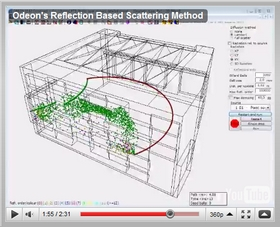
\includegraphics[scale=0.8]{figuras/odeon}
\caption{Tela de simulação 3D do Odeon$ ^{8} $}
\label{odeon}
\end{figure}

Este simulador foi utilizado como base e inspiração para o projeto proposto neste trabalho.

\subsection{AcMus}

O AcMus\footnote{\url{http://gsd.ime.usp.br/acmus/menu.html}} é um projeto voltado para a pesquisa sobre acústica musical que visa desenvolver modelos e ferramentas computacionais para o estudo de ambientes destinados à escuta musical. Este pretende ser o primeiro projeto de um núcleo de pesquisa interdisciplinar voltado para o assunto da acústica musical, nascido de um trabalho conjunto entre os departamentos de Música e Ciência da Computação da Universidade de São Paulo.

O AcMus é uma ferramenta de software livre implementado como um arcabouço orientado a objetos utilizando a linguagem de programação Java. A ferramenta reúne, em um único ambiente integrado, medição, análise e simulação acústica de salas.

A interface gráfica da ferramenta é baseada no template da IDE Eclipse, descrita na seção \ref{Eclipse}, conforme pode ser visto na figura \ref{acmus}. 

\begin{figure}[!htb]
\centering
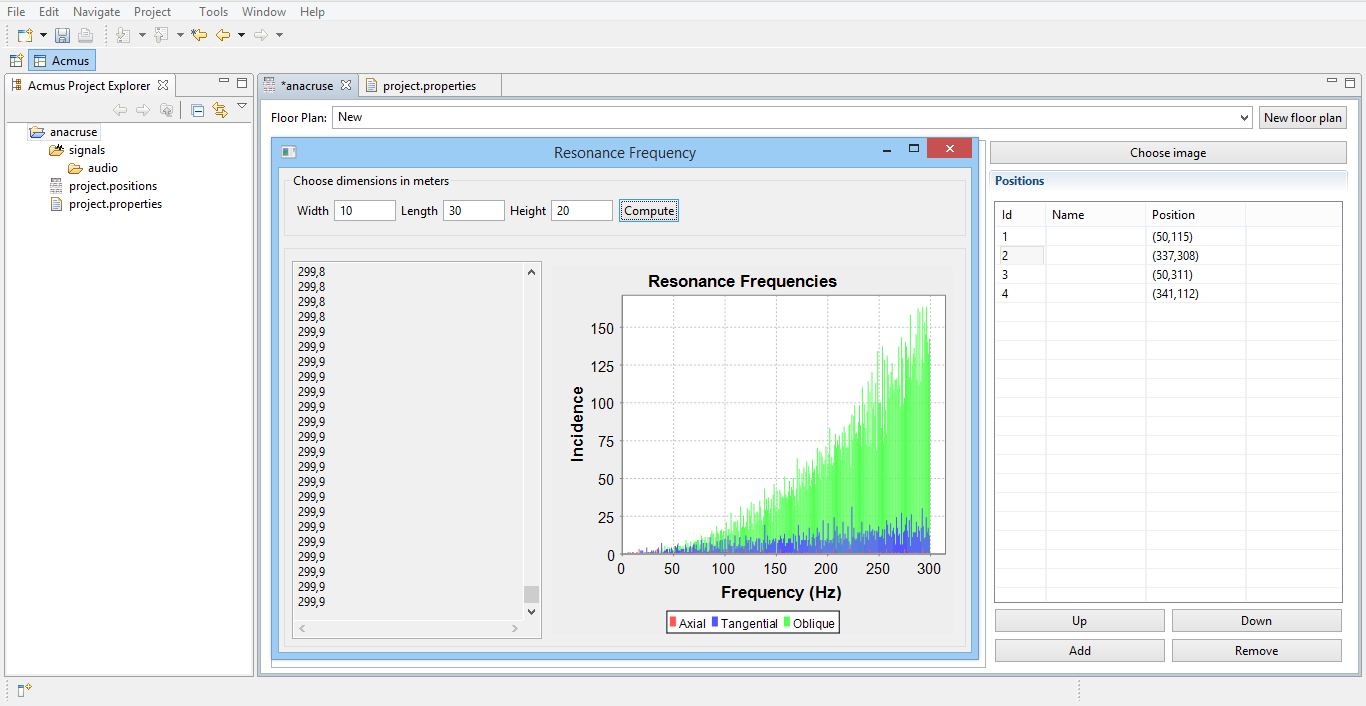
\includegraphics[scale=0.4]{figuras/acmus}
\caption{Telas de interface gráfica do software AcMus$ ^{9} $}
\label{acmus}
\end{figure}

\section{Considerações finais}

As ferramentas de desenvolvimento citadas neste capítulo são importantes tanto para o desenvolvimento da prova de conceito quanto do simulador em si. Em conjunto, essas ferramentas auxiliam o desenvolvimento de um sistema extensível e manutenível, visando qualidade e boas práticas de programação.

As ferramentas de simulação acústica descritas auxiliaram na compreensão do domínio do problema. Essas ferramentas foram investigadas com intuito de verificar quais são os sistemas existentes no mercado e como a simulação acústica é tratada nessas ferramentas. O estudo desses simuladores serviu de insumo para a elaboração da proposta do simulador acústico, produto de trabalho deste TCC.

